\documentclass[14pt, oneside]{article}

\title{ \textbf{Design \& Analysis of Algorithms} \\
Fractional Greedy Knapsack Investigation}
\author{ Axel Solano}

\usepackage{geometry}                		% See geometry.pdf to learn the layout options. There are lots.
\geometry{a4paper}                   		% ... or a4paper or a5paper or ...
%\geometry{landscape}                		% Activate for rotated page geometry
%\usepackage[parfill]{parskip}    		% Activate to begin paragraphs with an empty line rather than an indent
\usepackage{graphicx}				% Use pdf, png, jpg, or eps§ with pdflatex; use eps in DVI mode
\usepackage{float}
								% TeX will automatically convert eps --> pdf in pdflatex
\usepackage{amssymb}
\usepackage{amsmath}
\usepackage{listings}



\begin{document}
\pagenumbering{gobble}
\maketitle
\pagenumbering{arabic}
\tableofcontents
\newpage


 \section{Introduction}

In this program, I am going to use the scientific method to demonstrate that Fractional Greedy Knapsack Algorithm runs in O(n log(n)) time.


\section{Analysis of the Fractional Knapsack Problem}

\subsection{Heap Class:}
My heap is going to store each item with the key as the value of benefit/weight. I make the division because I want to find the greedy choice each time I store or remove an item. I create a class called "Val" which represent the item with the key as as the value of benefit/weight. Also, I create a function called "build" which create the heap to store the items in O(n). In this data structure, each time, it will remove the item with the greatest benefit and it will take O(log n) time.

\subsubsection{Build Function - Theoretical Analysis}

The build function check from the bottom of the tree to the top and the number of operations in each node is equivalent to the distance between the current level of the tree and the last level. The last level of the tree is founded on the nodes after the division by two of the total number nodes of the tree. In this theoretical analysis, I assume that the operations of each node are in the worst case scenario.

$$\sum_{i=1}^{h} 2^{h-i} i$$\\
\\
Reducing the expression

$$\sum_{i=1}^{h} 2^{h-i} i = 2^{h} \sum_{i=1}^{h} \frac{i}{2^{i}} $$

$$\sum_{i=1}^{h} \frac{i}{2^{i}}  = 1 + \sum_{j=1}^{h-1} \frac{1}{2^{j}}  - \frac{h}{2^{h+1}}$$

$$1 + \sum_{j=1}^{h-1} \frac{1}{2^{j}}  - 2^{\frac{h}{2^{h+1}}} = 1 + 1 - \frac{1}{2^{h-1}}  - \frac{h}{2^{h+1}}$$

$$ 2^{h} \sum_{i=1}^{h} \frac{i}{2^{i}} = 2^{h} [2 - \frac{1}{2^{h-1}}  - \frac{h}{2^{h+1}} ]$$

$$\sum_{i=1}^{h} 2^{h-i} i =  2^{h} \sum_{i=1}^{h} \frac{i}{2^{i}} = 2^{h+1} - 2 - \frac{h}{2} $$

Then, make the h = log(n/2) where n is equal to the number of nodes. Therefore, the build function has the equation of:

$$T(n) = n - \frac{log(n)}{2} - 3 $$

This equation can be reduced in Big-Oh notation as O(n).


\subsubsection{Build Function - Empirical Analysis}

In this analysis, I test my build function with the size from 10000 to 1000000 and for every case of the size I run 10 times, and then make an average of the time. In addition, I am going to use statistical analysis using the software R.

\paragraph{Fitting the points using linear regression}

$$ TIME = -2.017e-03 + 3.150e-07*SIZE $$
$$ p-value: < 2.2e-16 $$
$$ RSE: 0.004646 $$
$$ R^{2}:  0.9974 $$
$$ F-statistic: 3.83e+04 $$

\begin{figure}[H]
\centering
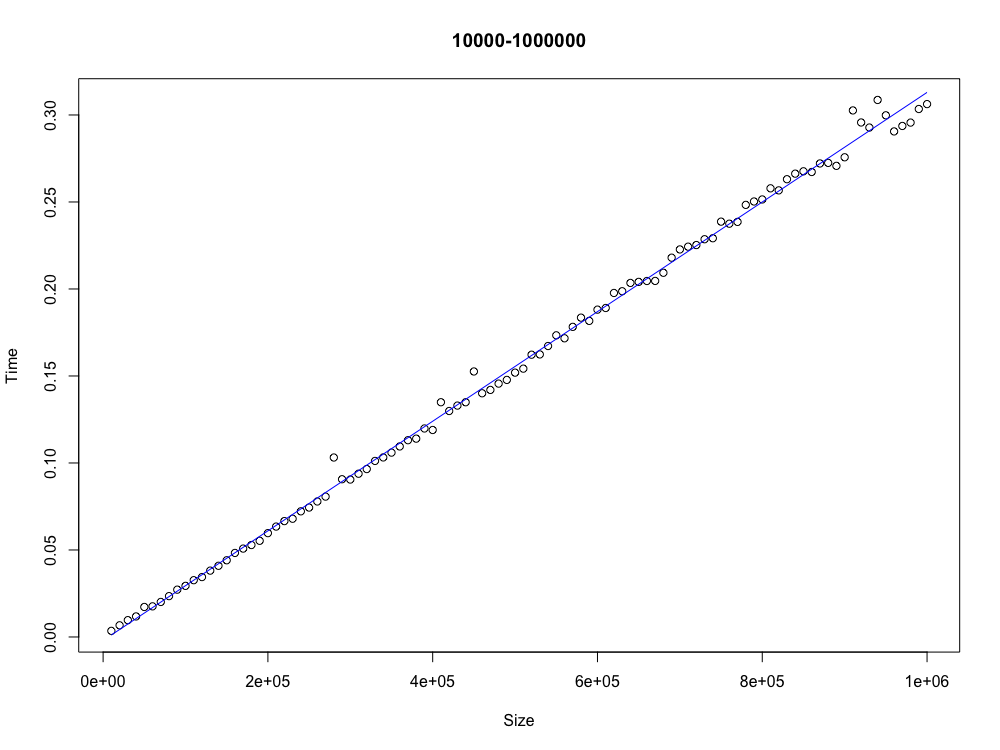
\includegraphics[width=\linewidth]{Rplot.png}
\caption{Linear Regression}
\end{figure}

\paragraph{Fitting the points using Polynomial regression of grade 2}
$$ TIME = -2.161687e-03 + 3.158481e-07*SIZE  -8.453501e-16*SIZE^{2}$$
$$ p-value: < 2.2e-16 $$
$$ RSE: 0.004669 $$
$$ R^{2}:  0.9974 $$
$$ F-statistic: 1.896e+04 $$

\begin{figure}[H]
\centering
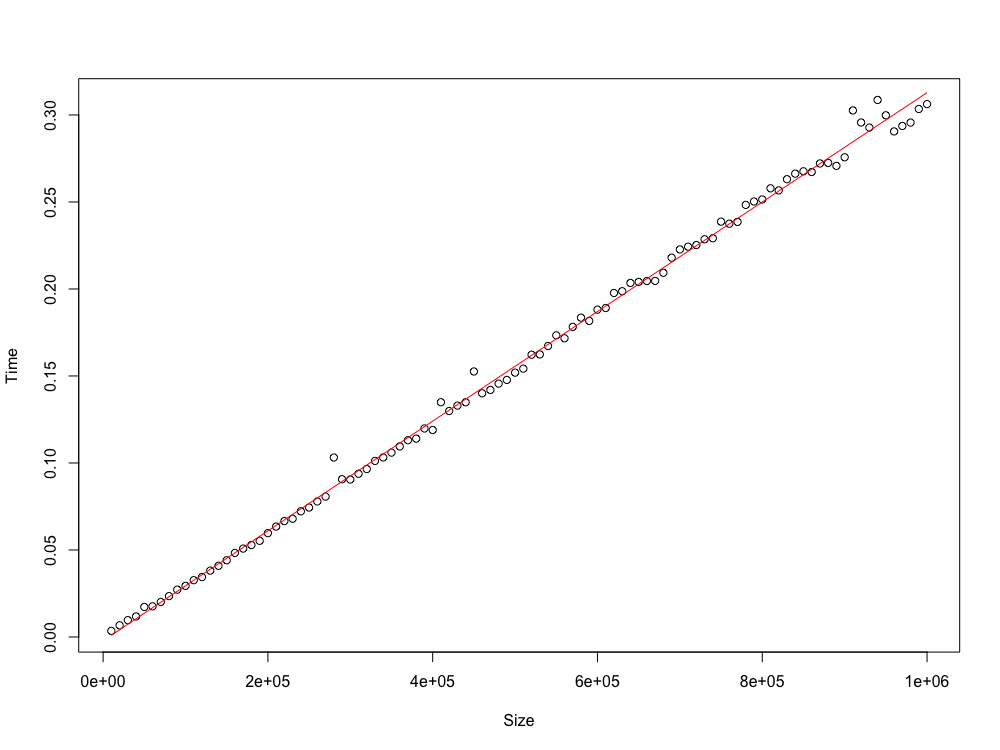
\includegraphics[width=\linewidth]{Rplot01.png}
\caption{Polynomial regression of grade 2}
\end{figure}

\paragraph{Fitting the points using Polynomial regression of grade 3}
$$ TIME = (1.445568e-03 ) + (2.740265e-07)*SIZE  +(1.021602e-13 )*SIZE^{2} + (-6.799047e-20)*SIZE^{3}$$
$$ p-value: < 2.2e-16 $$
$$ RSE: 0.004507 $$
$$ R^{2}:  0.9976 $$
$$ F-statistic: 1.357e+04$$

\begin{figure}[H]
\centering
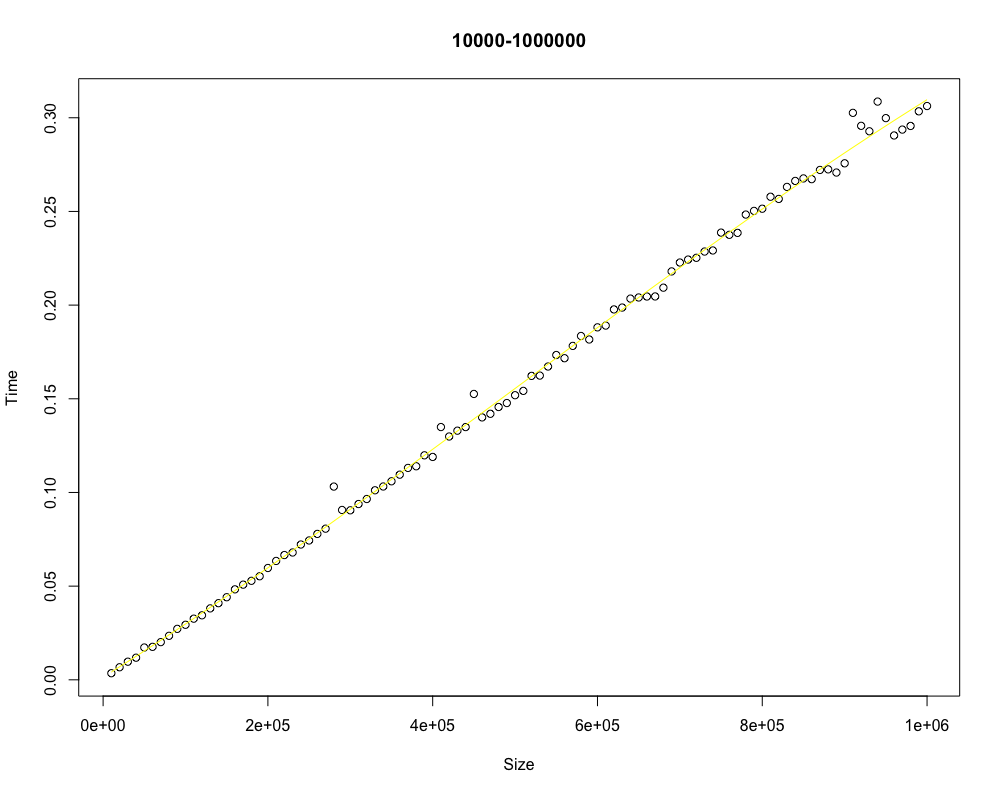
\includegraphics[width=\linewidth]{Rplot02.png}
\caption{Polynomial regression of grade 3}
\end{figure}

\paragraph{Fitting the points using Polynomial regression of grade 4}
$$ TIME = (-1.096532e-03 ) + ( 3.222104e-07)*SIZE  +(-1.100373e-13)*SIZE^{2} + (2.577337e-19)*SIZE^{3} + (-1.612496e-25)*SIZE^{4}$$
$$ p-value: < 2.2e-16 $$
$$ RSE: 0.004462 $$
$$ R^{2}:  0.9977 $$
$$ F-statistic: 1.039e+04$$

\begin{figure}[H]
\centering
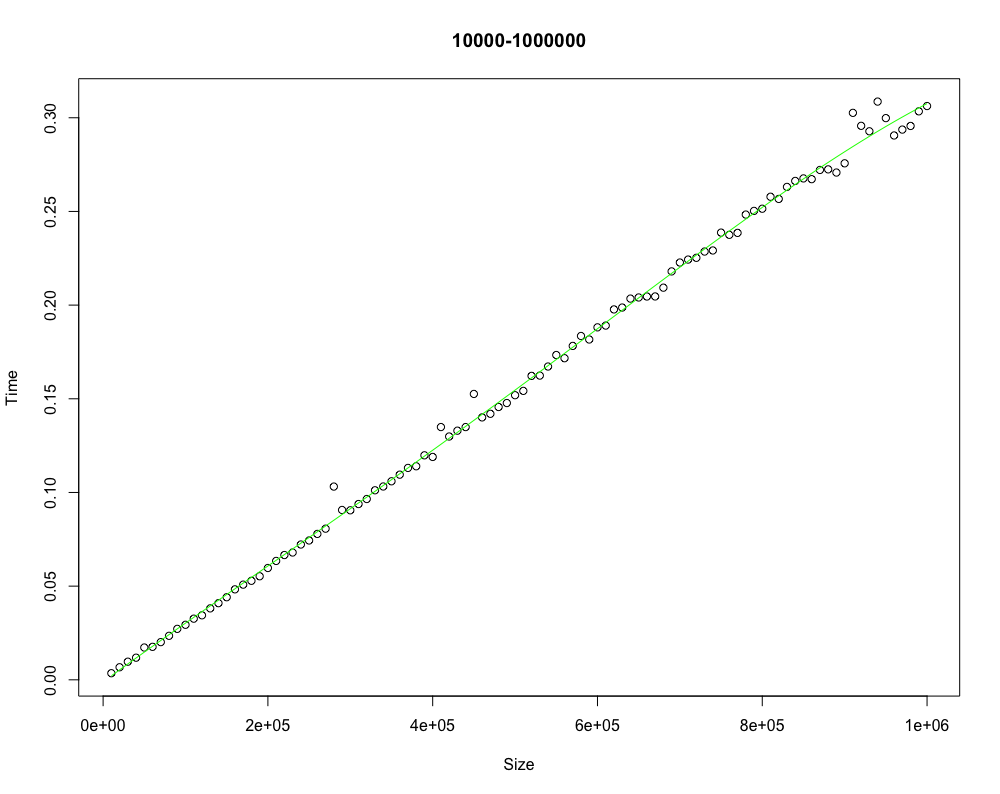
\includegraphics[width=\linewidth]{Rplot03.png}
\caption{Polynomial regression of grade 4}
\end{figure}

In conclusion, the best option is the linear regression because its F-statistic is greater than the others. I use the F-statistic because the p-value is really small in all the test, the Residual standard error are very similar and the $R^{2}$  is near to 1 in all tests, therefore, the only variable to differentiate is the F-statistic which confirm that there is a strong relationship as a linear model. As a result, this linear model confirm my theoretical claim of O(n).


\subsection{Knapsack Class:}

\subsubsection{Testing the algorithm:}
In this analysis, I test my knapsack function with the size from 10000 to 1000000 and for every case of the size I run 10 times, and then make an average of the time. In addition, I am going to use statistical analysis using the software R.Also, I create a variable called sum which represent the summation of each weight of the item; I create this variable to use in my test as the input of the maximum weight. In the test, I put the maximum weight as the total weight, therefore, I am indirectly sorting the items and testing the same time the worst case scenario. I did the previous implementation to prove that my function runs in O(nlogn).

\paragraph{Fitting the points using linear regression}

$$ TIME = (-4.025736e-01) + (9.524633e-06 )*SIZE $$
$$ p-value: < 2.2e-16 $$
$$ RSE: 0.1794 $$
$$ R^{2}:  0.9958 $$
$$ F-statistic: 2.348e+04 $$

\begin{figure}[H]
\centering
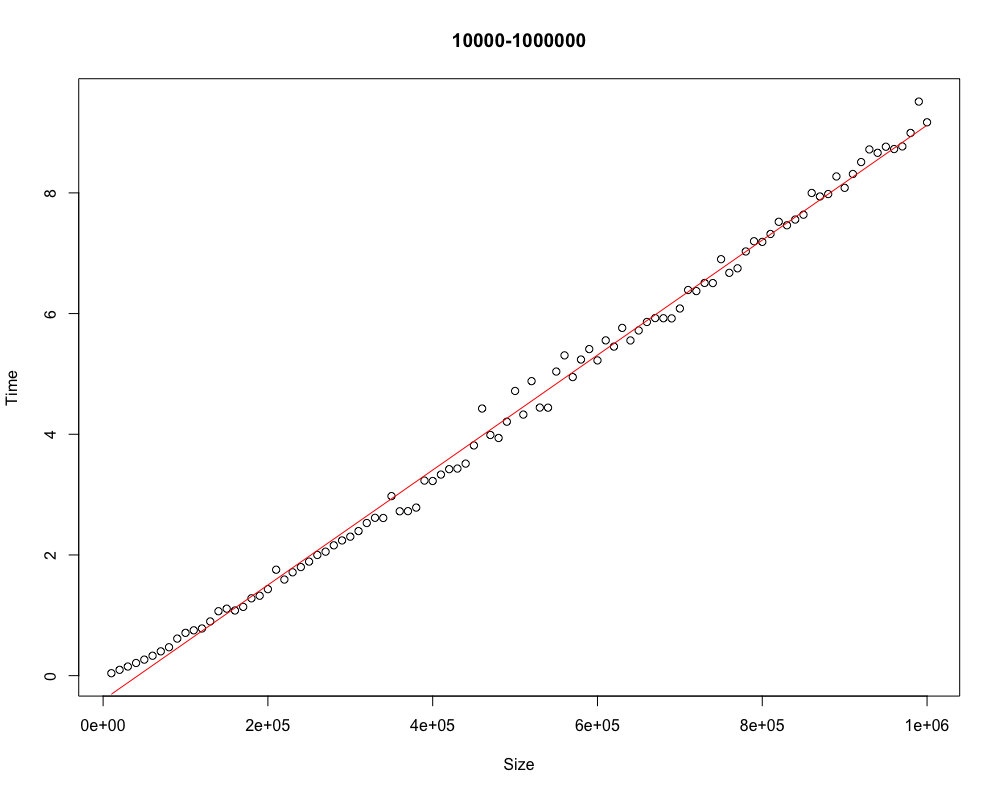
\includegraphics[width=\linewidth]{Rplot04.png}
\caption{Linear Regression}
\end{figure}


\paragraph{Fitting the points using Polynomial regression of grade 2}
$$ TIME = (-2.060008e-01) + (8.368323e-06)*SIZE  - (1.144862e-12)*SIZE^{2}$$
$$ p-value: < 2.2e-16 $$
$$ RSE: 0.1582  $$
$$ R^{2}:  0.9968 $$
$$ F-statistic: 1.512e+04$$

\begin{figure}[H]
\centering
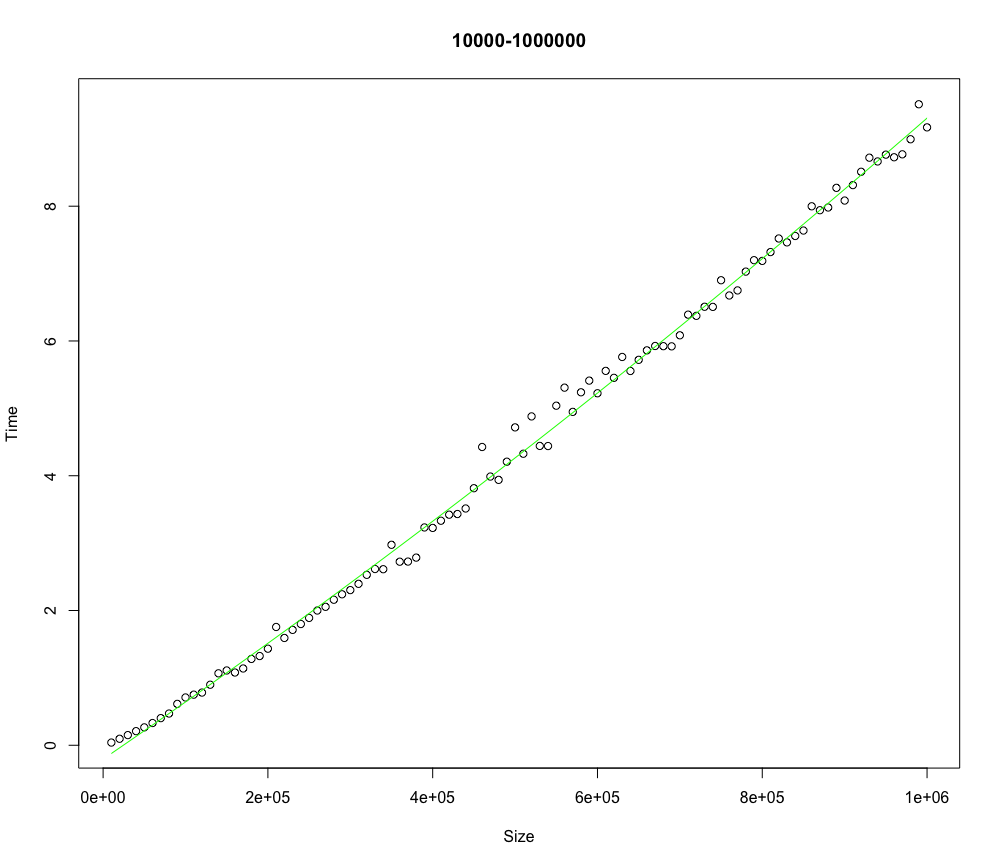
\includegraphics[width=\linewidth]{Rplot06.png}
\caption{Polynomial regression of grade 2}
\end{figure}

\paragraph{Fitting the points using Polynomial regression of grade 3}
$$ TIME = (-8.914651e-02) + (7.013543e-06 )*SIZE  +(4.481650e-12)*SIZE^{2} + (-2.202501e-18)*SIZE^{3}$$
$$ p-value: < 2.2e-16 $$
$$ RSE:  0.1532$$
$$ R^{2}:  0.997 $$
$$ F-statistic:  1.074e+04$$

\begin{figure}[H]
\centering
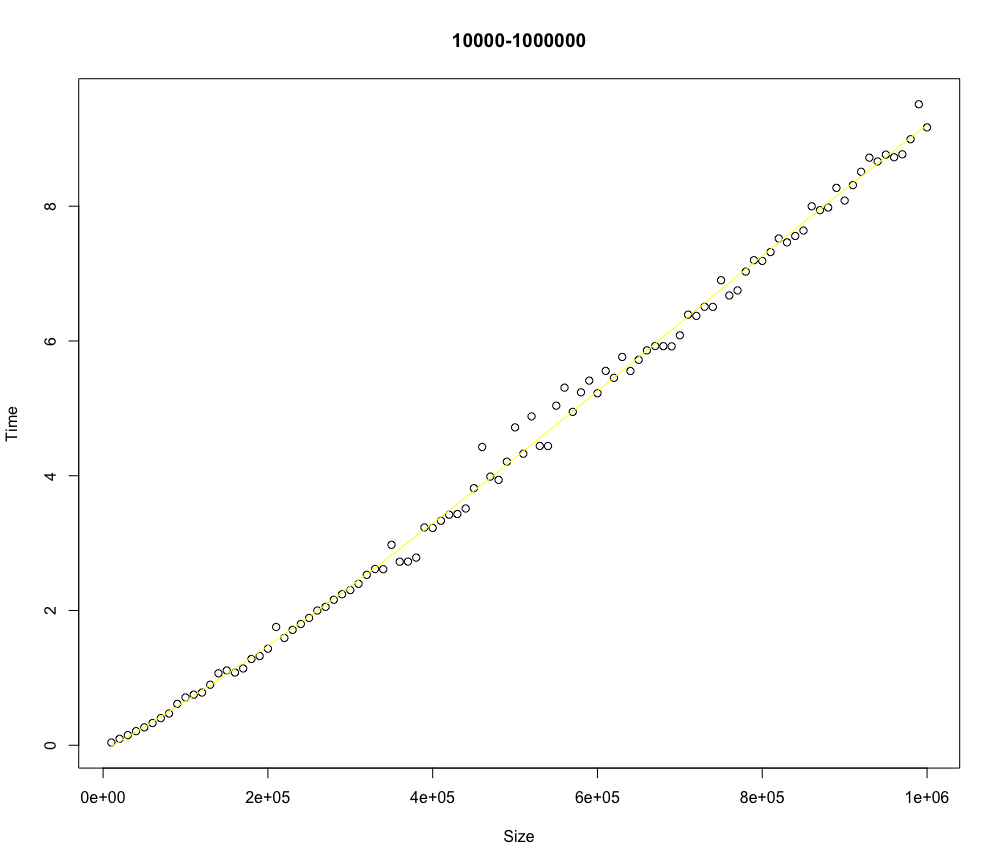
\includegraphics[width=\linewidth]{Rplot07.png}
\caption{Polynomial regression of grade 3}
\end{figure}

\paragraph{Fitting the points using Polynomial regression of grade 4}
$$ TIME = (2.749202e-02) + ( 4.802733e-06)*SIZE  +(1.421785e-11 )*SIZE^{2} + (-1.714762e-17)*SIZE^{3} + ( 7.398573e-24 )*SIZE^{4}$$
$$ p-value: < 2.2e-16 $$
$$ RSE: 0.1498 $$
$$ R^{2}:  0.9972 $$
$$ F-statistic: 8437$$

\begin{figure}[H]
\centering
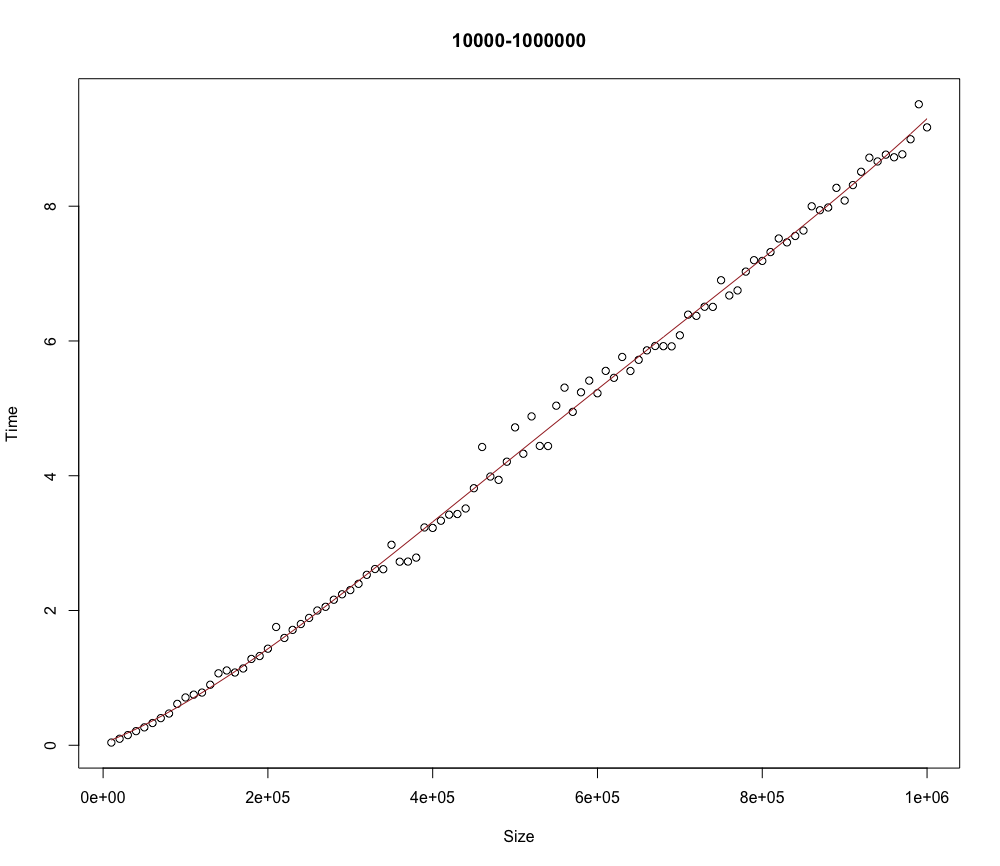
\includegraphics[width=\linewidth]{Rplot08.png}
\caption{Polynomial regression of grade 4}
\end{figure}

\paragraph{Fitting the points using Polynomial regression of grade 5}
$$ TIME = (-4.112013e-02) + ( 6.707867e-06 )*SIZE  +(1.275650e-12  )*SIZE^{2} + ( 1.676458e-17 )*SIZE^{3} + (-3.027888e-23 )*SIZE^{4} + (1.492176e-29  )*SIZE^{6}$$
$$ p-value: < 2.2e-16 $$
$$ RSE: 0.1494$$
$$ R^{2}:  0.9972 $$
$$ F-statistic: 6779$$

\begin{figure}[H]
\centering
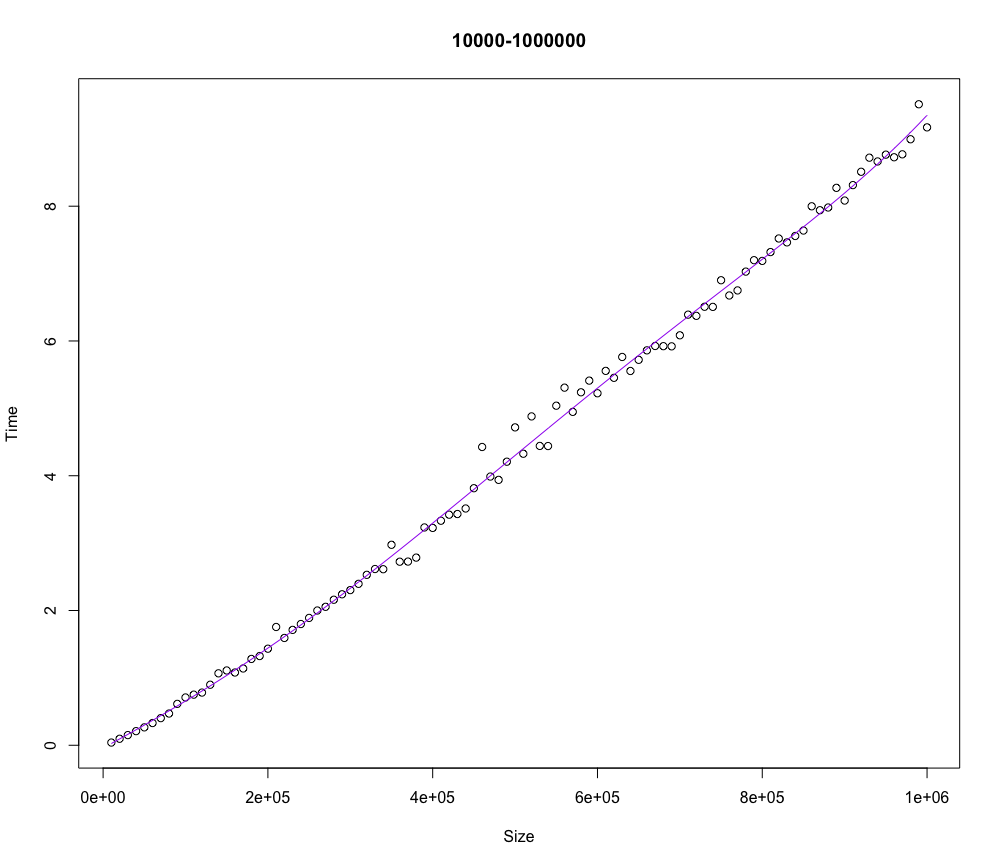
\includegraphics[width=\linewidth]{Rplot09.png}
\caption{Polynomial regression of grade 5}
\end{figure}

\paragraph{Fitting the points using n*log(n) curve}

$$ TIME = -(1.713231e-01) + (4.717935e-07)*SIZE *log(SIZE)$$
$$ p-value: < 2.2e-16 $$
$$ RSE: 0.1552$$
$$ R^{2}:  0.9969$$
$$ F-statistic: 3.142e+04$$

\begin{figure}[H]
\centering
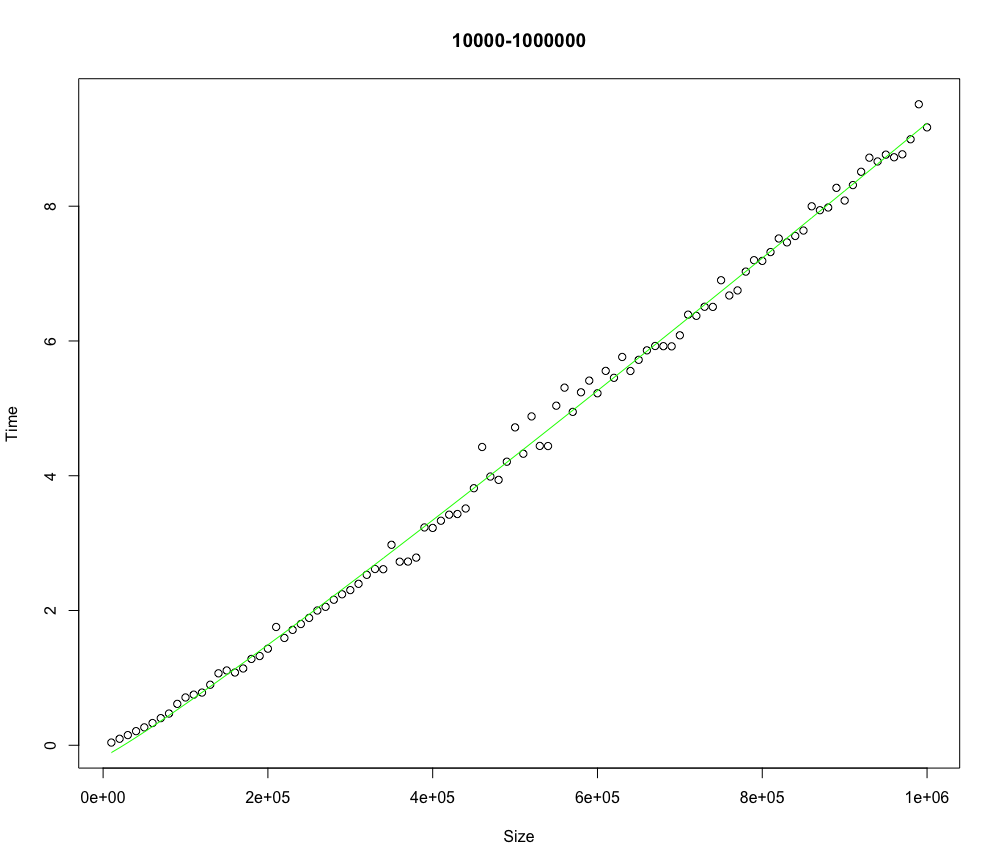
\includegraphics[width=\linewidth]{Rplot05.png}
\caption{nlogn style}
\end{figure}

\paragraph{Fitting the points using n*log(n) curve with addition of two functions}

$$ TIME =  (-1.591273e-01 ) + (4.963666e-07)*(SIZE*log2(SIZE) - SIZE - log2(SIZE))$$
$$ p-value: < 2.2e-16 $$
$$ RSE: 0.1546$$
$$ R^{2}:  0.9969$$
$$ F-statistic: 3.167e+04$$

\begin{figure}[H]
\centering
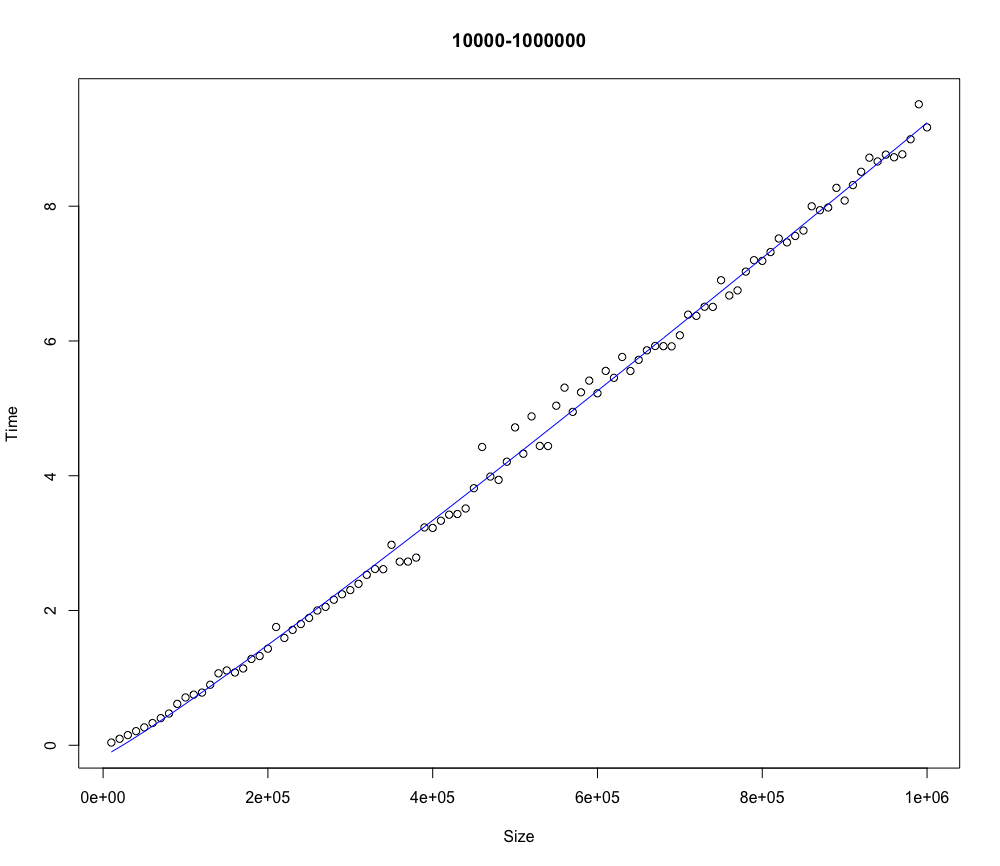
\includegraphics[width=\linewidth]{Rplot10.png}
\caption{nlogn style}
\end{figure}

In conclusion, the best option is the last model which math with the Big-Oh notation O(nlogn) because its F-statistic is the greatest of all the model. The variable F-statistic helps in the analysis of choosing the best fit model
when the other math models present similar RSE, similar $R^{2}$ and the p-value. All the models have a p-value less than 0.05, in fact, all the p-values are really low but the major point about this fact is that the coefficients
become lower every time there is an increase in the polynomial model and in each increase the F-statistic is not increasing, therefore it is not appropriate to choose those other models.


\end{document}
